\chapter{The Impact Parameter Method} % Main chapter title

\label{Chapter5} % For referencing the chapter elsewhere, use \ref{Chapter1} 

In Chapter \ref{Chapter4} one has studied the influence of the primary vertex uncertainty on the dataset. In the following, a new way of finding the impact parameter vector is going to be proposed and compared to the tangential approach \parencite{Claudia_thesis} currently in use by the \verb|Artus| framework.

\section{Theoretical background}
First of all, one has to find the track of the particle and a suitable parametrisation thereof. Since we are considering charged particles moving with a velocity \textbf{v} in a homogeneous magnetic field $\boldsymbol{B} = B\boldsymbol{e}_z$, one expects to find a helical trajectory. Evidently, cylindrical coordinates are the most elementary way to parametrize it, keeping the problem as simple as possible. In the following, a quick derivation of the trajectory is going to be discussed, since the parameters appearing in the equations of motion have to be uniquely identified with those used by the track fitting algorithm.\\
In order to find the track, consider a classical particle of charge $q$ as described above. On such a particle, the relativistic Lagrangian $\mathcal{L}$ (up to a gauge transformation) takes in cgs-Gaussian units the form \parencite{Jackson}
\begin{equation}
	\mathcal{L} = -mc^2\cdot\sqrt{1-\left(\frac{\dot{\boldsymbol{x}}}{c}\right)^2}+\frac{q}{c}( \boldsymbol{v}\cdot\mathbf{A})
\end{equation}
with the vector potential $\boldsymbol{A}$ satisfying $\boldsymbol{B} = \nabla \times \mathbf{A}$. In case of a homogeneous magnetic field, $\boldsymbol{A}$ can be written (up to a gauge transformation) as
\begin{equation}
	\mathbf{A} = \frac{B}{2}\left(\begin{tabular}{c}
	$-y $\\ 
	$x$\\ 
	$0$
	\end{tabular} \right)
\end{equation}
leading to the Lagrangian
\begin{equation}
	\mathcal{L} = -mc^2\cdot\sqrt{1-\left(\frac{\dot{\boldsymbol{x}}}{c}\right)^2}+\frac{qB}{2c}( x\dot{y} - y\dot{x}),
\end{equation}
which can be rewritten in SI units as
\begin{equation}
	\mathcal{L} = -mc^2\cdot\sqrt{1-\left(\frac{\dot{\boldsymbol{x}}}{c}\right)^2}+\frac{qB}{2}( x\dot{y} - y\dot{x}).
\end{equation}\\
Using the variational principle, the action $S =\int\mathcal{L}dt$ is stationary if and only if $\mathcal{L}$ fulfils the Euler-Lagrange equations yielding the following set of equations of motion:
\begin{center}
	$\left\lbrace
	\begin{aligned}
		-qB\dot{x}&=m\gamma\ddot{y}\\
		qB\dot{y}&=m\gamma\ddot{x}\\
		0&=mg\ddot{z}
	\end{aligned}
	\right.$
\end{center}
where $\gamma$ denotes the Lorentz-gamma. The ansatz
\begin{equation}
	\boldsymbol{x}(t) = \boldsymbol{O'} +  \left(\begin{tabular}{c}
	$R\cos(\omega t + \varphi_1) $\\ 
	$-R\sin(\omega t + \varphi_1) $\\ 
	$v_z t $
	\label{eq:ansatz}
	\end{tabular} \right)
\end{equation}
(where \textbf{O'} is a constant vector) is indeed a solution to the problem. Putting this ansatz in the equations of motion provides the correspondence between the magnitude of the elements of the 4-momentum $p^\mu$, the particle charge $q$ and the geometrical parameter $\omega$, the angular frequency given by $\omega = \frac{qB}{m\gamma}$. Considering the magnitude of the relativistic 3-momentum of a such particle yields the expression between the radius $R$ and $p$, given by $R=\frac{p_T}{qB}=\frac{p\sin\theta}{qB}$, where $\theta$ denotes the polar angle.\\
Having expressed $R$ and $\omega$ through the measurable physical variables $p, B$ and $m\gamma$ (which can be derived from the total energy of the particle), now one can move to the helix reconstruction algorithm, which executes a fit with respect to the following parameters:
\begin{itemize}
	\item $\frac{q}{p}$: the signed inverse of the momentum at a reference point \textbf{R} $=(R_x, R_y, R_z)$ defined as the closest point on the helix to the center of the detector
	\item $\lambda = \frac{\pi}{2} - \theta$ ; $\lambda \in [0, \pi)$: the polar angle of the 3-momentum in \textbf{R} to XY-plane
	\item $\varphi \in [-\pi,\pi)$: the azimuth angle of the 3-momentum vector in the point \textbf{R} in the XY-plane with respect to the x-axis
	\item $d_{xy} = -R_x \sin\varphi + R_y \cos\varphi$: the signed distance between the tangent of the helix in \textbf{R} and the origin in the XY-plane
	\item $d_{sz} = R_z\cos\lambda - (R_x\cos\varphi+R_y\sin\varphi)\sin\lambda$: defined in the SZ-plane, where S denotes to the distance travelled by the particle in the XY-plane
\end{itemize}
A visualisation of these parameters can be found in Fig. \ref{fig:geometry}, where $v$ corresponds to the primary vertex of $\tau$-production (which is with a very good approximation the same as the production vertex of the Higgs-boson) and $\boldsymbol{O'}$ is the projected rotation axis of the helix. By using the above parametrisation, one has also to take into account that $\varphi_1$ is positive in the negative $\varphi$ region; this has the advantage that positively charged particles move to the direction of increasing $\varphi_1$. Obviously, one could have taken a trigonometric argument of the form $(\omega t-\varphi_1)$ with an oppositely signed angle $\varphi_1$ -- this is just matter of convention.
\begin{figure}[h]
	\centering
	\begin{tikzpicture}
	\centering
	
	\def\centerarc[#1](#2)(#3:#4:#5)% Syntax: [draw options] (center) (initial angle:final angle:radius)
	{ \draw[#1] ($(#2)+({#5*cos(#3)},{#5*sin(#3)})$) arc (#3:#4:#5); }
	
	\draw[thick,->, name path = x_axis_line] (-1,0) -- (10,0) node[anchor=north west] (x_axis) {x};
	\draw[thick,->] (0,-1) -- (0,4) node[anchor=south east] {y};
	\fill (0,0) circle (2pt) node[anchor=north east]{O};
	%\draw [name path = c] (8,6) circle (4);
	\centerarc[name path = c](8,6)(170:260:6);
	\path [name path = Op,draw] (0,0) -- (8,6) coordinate (Op_point);
	\node[anchor=north] at (2,1.5) {$d_{xy}$};
	\draw[dashed, name path = horizontal_Op] (7.5,6)--(10,6)  coordinate (horizontal_Op_line);
	\fill (8,6) circle (2pt) node[anchor=south]{O'};
	\fill [name intersections={of=Op and c}]
	(intersection-1) circle (2pt) node[anchor=east] {R} coordinate (R);
	\draw[dashed, name path = tangent_line] (intersection-1) --++(4,-5.33) coordinate (tangent);
	\draw[line width=0.6mm,->] (intersection-1) --++(0.5,-0.66) node [anchor=east] {$\boldsymbol{p}_T$};
	\draw[dashed] (intersection-1) --++(-3,4); %(3,-4)
	\fill [name intersections={of=tangent_line and x_axis_line}]
	(intersection-1) circle (0pt) coordinate[anchor=north east] (inter);
	\draw[dashed] (intersection-1) --++(-3,4);
	\pic [draw, <-, "$\varphi$", angle eccentricity=0.6,angle radius=11mm] {angle = tangent--inter--x_axis};
	%PV:
	\draw[->] (0,0) -- (2,3);
	\node[anchor=south] at (0.8,1.5) {$\boldsymbol{v}$};
	\pic [draw, <-, "$\varphi_1$", angle eccentricity=0.6,angle radius=5mm] {angle = R--Op_point--horizontal_Op_line};
	\end{tikzpicture}
	\caption{a visualisation of fit parameters, for a negatively charged particle in the XY-plane; here $\boldsymbol{v}$ is the PV-vector and $\varphi_1>0$ and $\varphi<0$}
	\label{fig:geometry}
\end{figure}\\
As introduced in section \ref{sec:IP_method} in the gluon-gluon fusion process, the impact parameter is a $CP$-sensitive variable enabling us to determine the angle $\varphi^*$. Nevertheless, a direct measure of this vector is not possible, hence it is necessary to calculate it, whereas multiple approaches can be considered. In this thesis, two of them are going to be discussed: the so-called tangential approximation \parencite{Claudia_thesis} and the helical approximation.\\

\section{The tangential approximation}
A typical particle produced in the CMS-experiment is highly relativistic, which leads to extremely great curvatures and radii $R$ compared to the scale of the IP. Therefore, one could approximate in the close neighbourhood in the region of the secondary vertex (the $\tau$-decay vertex) the helical trajectory with a straight line. Assuming the primary vertex is close to the centre of the detector (the origin) one could utilise the above introduced reference point \textbf{R} to extrapolate the trajectory linearly along $\lambda$ and $\varphi$.\\
\begin{figure}[h]
	\centering
	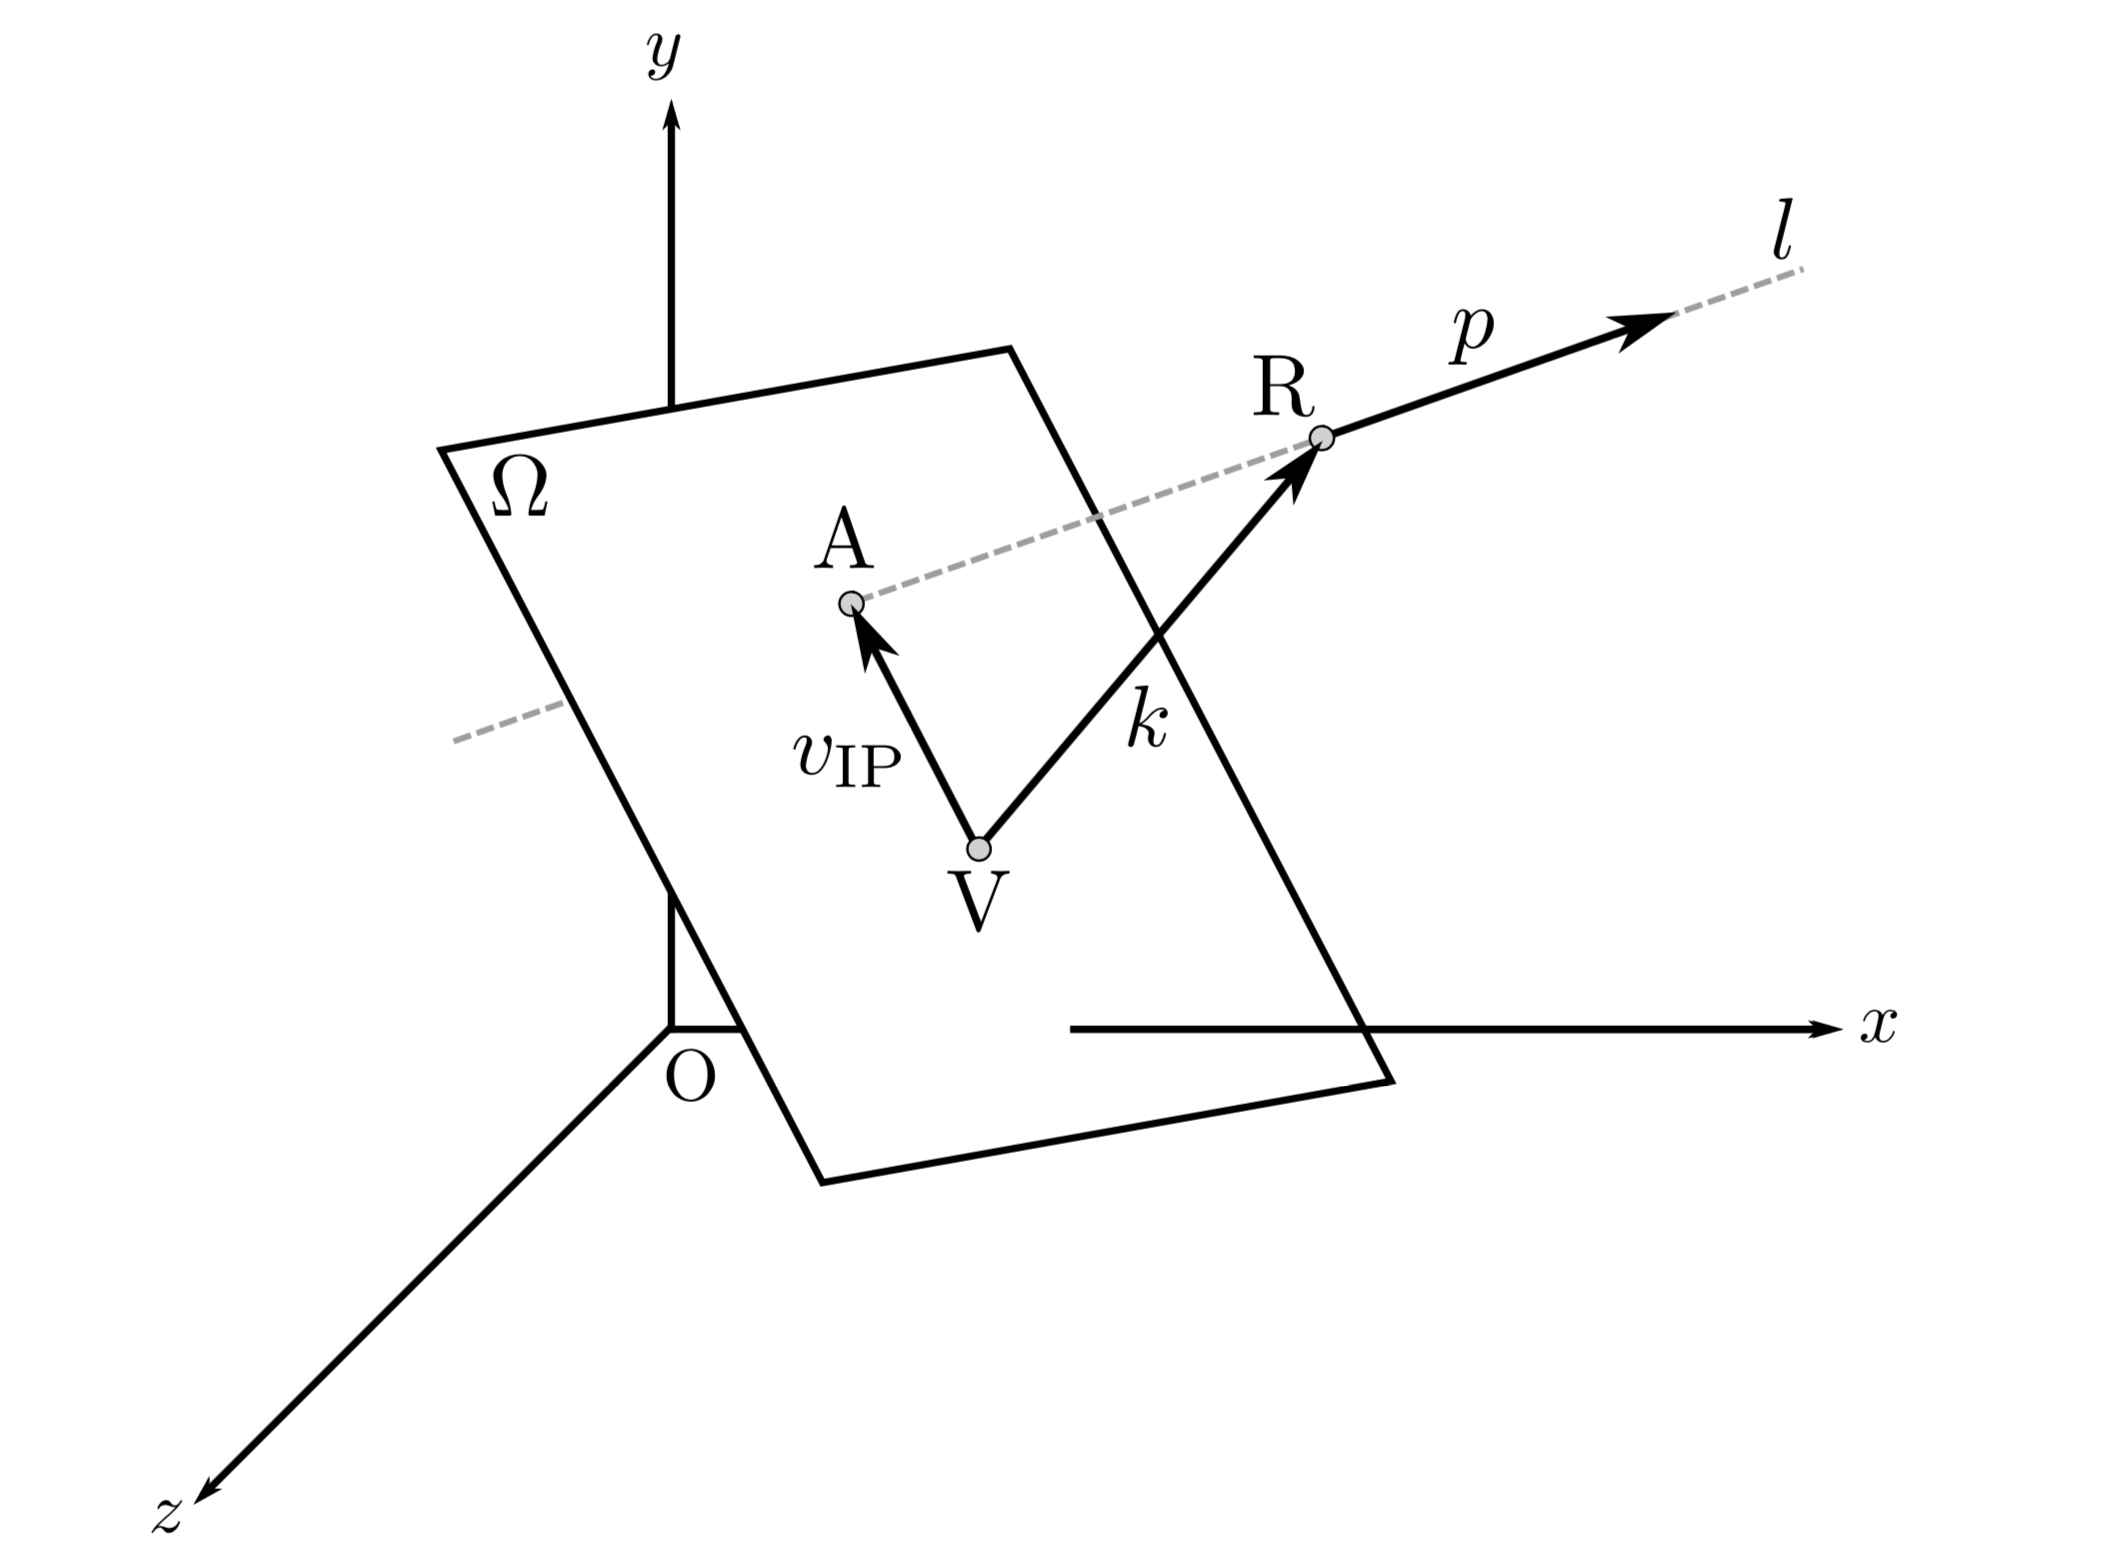
\includegraphics[width=0.5\linewidth]{Figures/IP_tangential}
	\caption{The geometry of finding the IP-vector (here denoted as $v_{IP}$). Source: \parencite{Claudia_thesis}}
	\label{fig:iptangential}
\end{figure}\\
To determine the IP with this method, consider Fig. \ref{fig:iptangential}, where V is the primary vertex. From the definition of the impact parameter follows that the distance between the straight line defined by the 3-momentum vector $\boldsymbol{p}$ of the lepton $l$ at \textbf{R} and the primary vertex point V should be minimised. In other terms, the IP-Vector $\boldsymbol{v}_{IP}$ should stay orthogonal to the (normalised) momentum vector $\boldsymbol{\hat{p}}$ meaning
\begin{equation}
	\boldsymbol{v}_{IP} \cdot \boldsymbol{\hat{p}} = 0.
\end{equation}
Nevertheless, the vector $\overrightarrow{VA}$ can be expressed as
\begin{equation}
	\overrightarrow{VA} = \boldsymbol{v}_{IP} = \boldsymbol{k}+\alpha \cdot \boldsymbol{\hat{p}},
\end{equation}
with an $\alpha \in \mathbb{R}$. Combining the two conditions yields
\begin{equation}
	\alpha = -\boldsymbol{k}\cdot\boldsymbol{\hat{p}}
\end{equation}
which then can be used to determine the $\boldsymbol{v}_{IP}$:
\begin{equation}
	\boldsymbol{v}_{IP} = \boldsymbol{k}-(\boldsymbol{k}\cdot\boldsymbol{\hat{p}})\boldsymbol{\hat{p}}
\end{equation}
There are however multiple problems with such an approach. First, it uses a physically meaningless point \textbf{R} to obtain a crucial physical parameter, $\boldsymbol{v}_{IP}$. Second, it does not take the curvature of the particle trajectory into account, leading to errors. Third, and most importantly, the basic assumption (about the position of the primary vertex) on which this algorithm lies upon, does not necessarily hold, see \ref{fig:PVs}. In this figure, one can immediately observe that the position of the primary vertices is of the same order of magnitude as the length of the impact parameter vectors (see \ref{fig:lambda_dist}). Therefore, a further study of IP-reconstruction needs to be considered.\\
\begin{figure}[h]
	\centering
	\subfigure{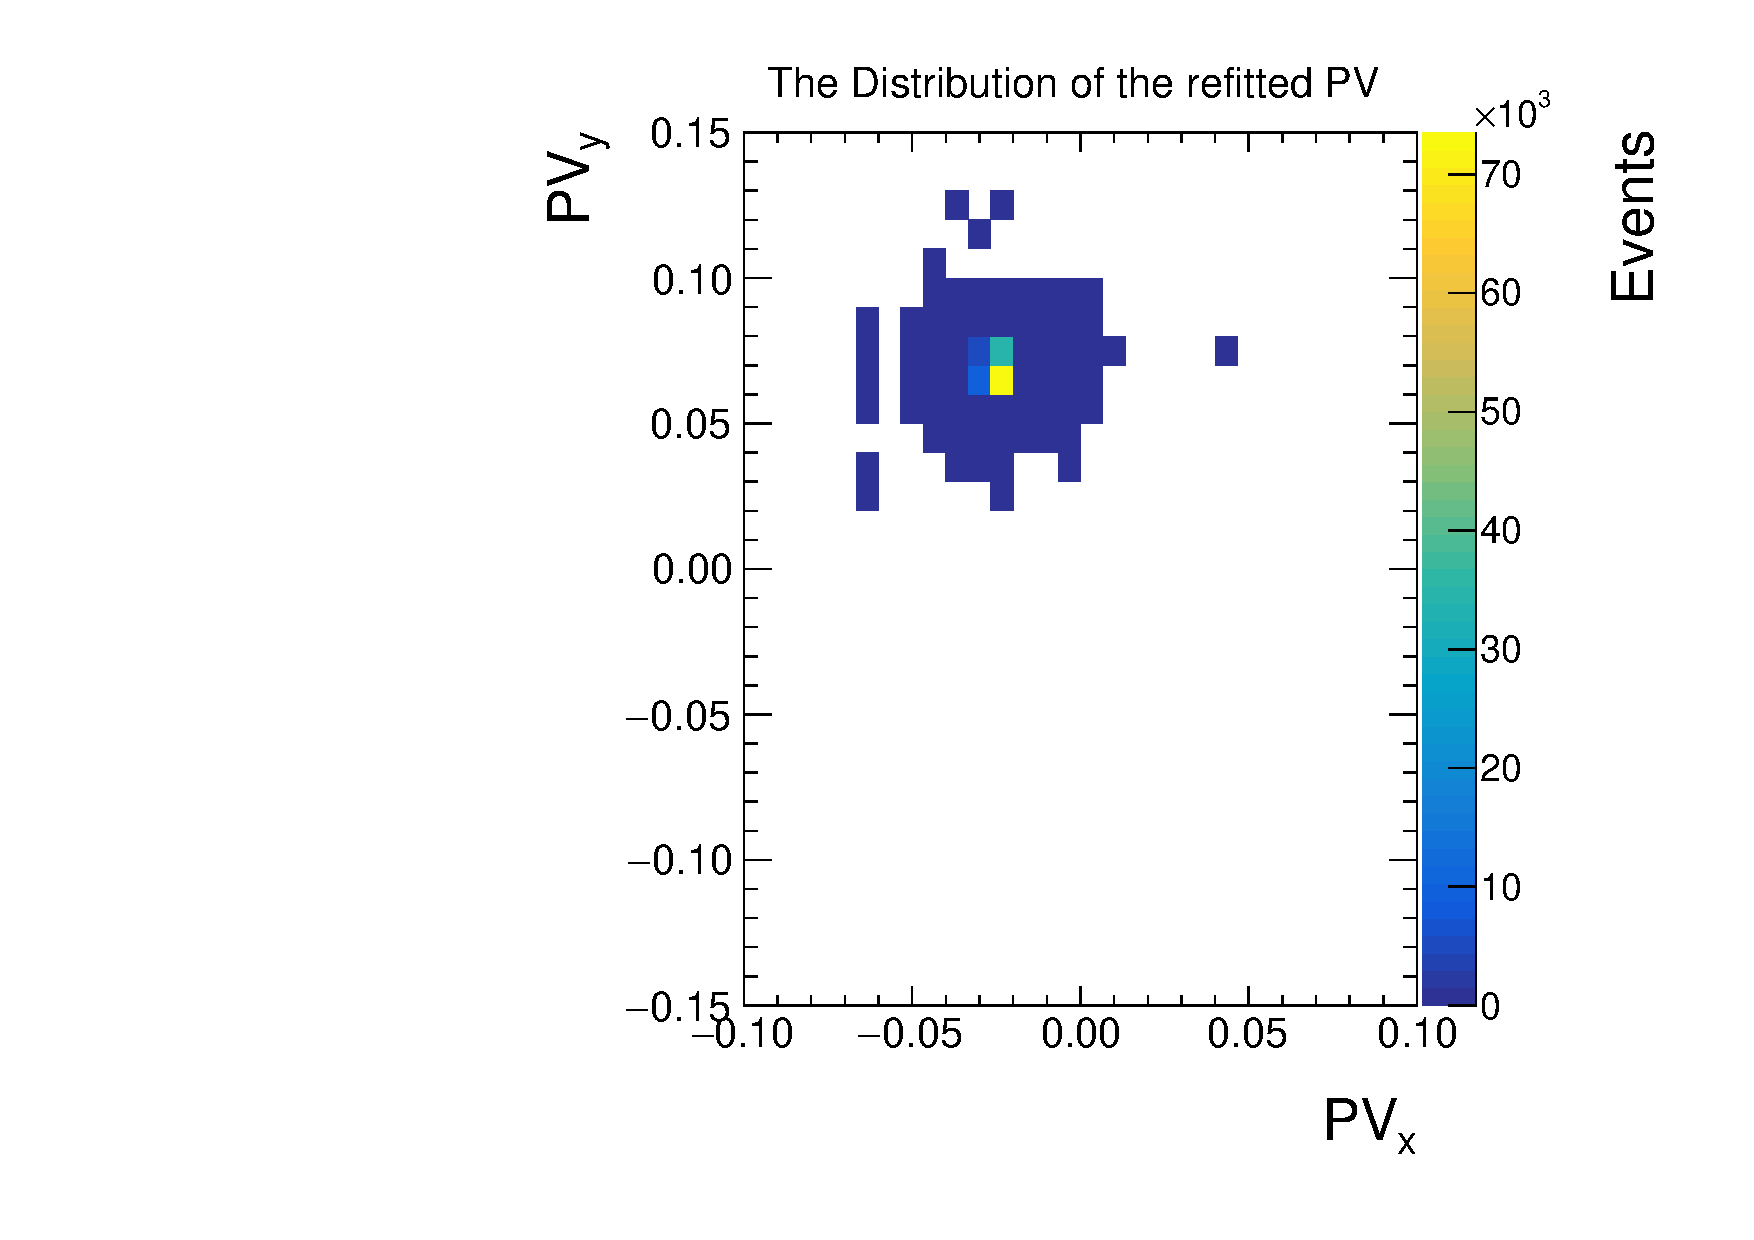
\includegraphics[width=0.4\linewidth]{Figures/PVs}}
	\subfigure{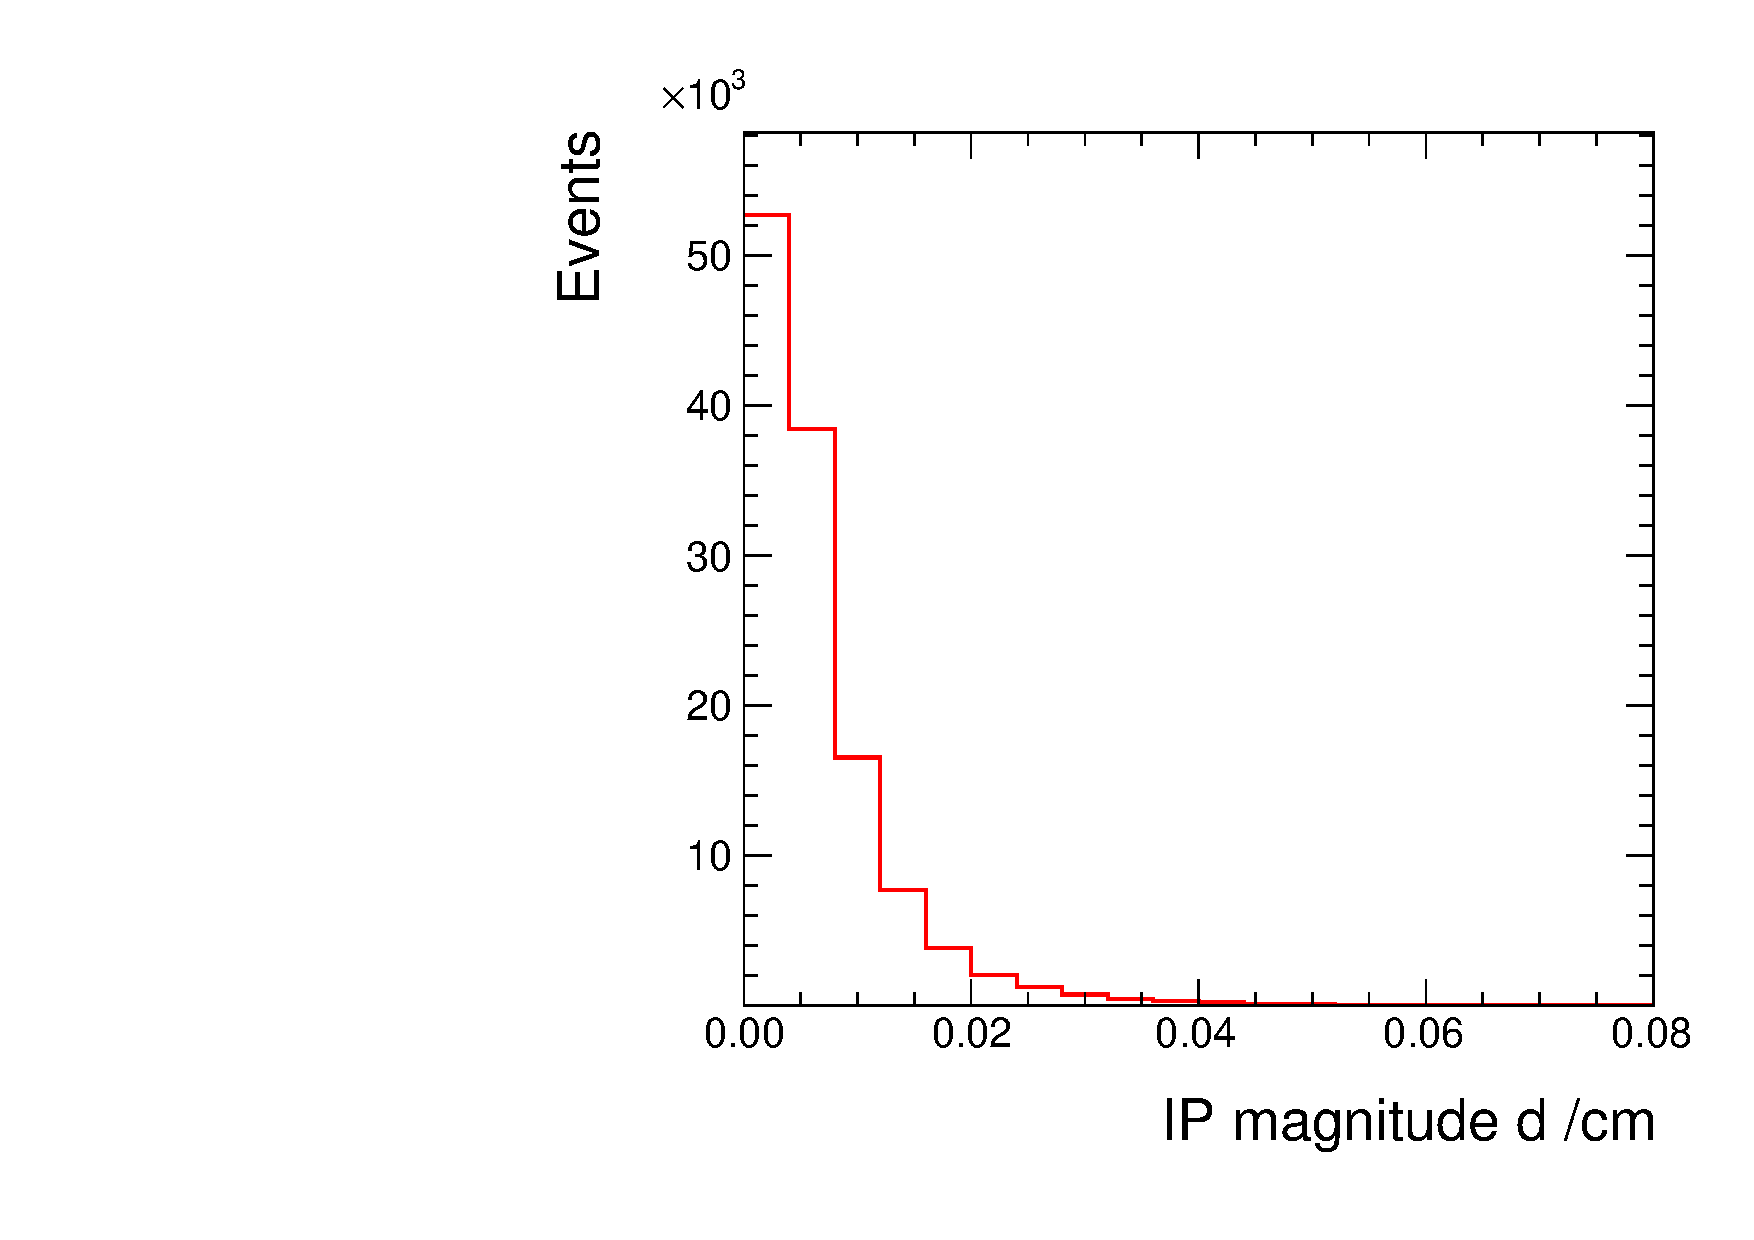
\includegraphics[width=0.4\linewidth]{Figures/IP_mag.pdf}}
	\caption{Left: The positions of the refitted primary vertices of the Higgs decays\\Right: The Distribution of IP-Magnitudes in all decay channels}
	\label{fig:PVs}
\end{figure}
\newpage
\section{The helical approximation}
Given the fact that both the $\tau$ particles and the secondary vertices cannot be precisely reconstructed, one needs to find a point which lies as closely to the latter, as possible. Another assumption is the consideration of the point of closest approach (PCA) of the particle on its trajectory as the base of IP-reconstruction. Having defined the IP-vector as the vector pointing from the primary vertex V to the PCA and considering the helix parametrised as in Eq. \ref{eq:ansatz}, it is simple to obtain the newly defined impact parameter, by minimising
\begin{equation}
	\delta(t) = |\boldsymbol{x}(t)-\boldsymbol{v}|^2,
\end{equation}
in $t$, where \textbf{v} denotes the vector pointing from the origin to V. Since $\delta(t)$ is a smooth function with existing higher-order derivatives, the problem can be  calculated numerically.
\subsection{Implementation}
Nevertheless, comparing the fit parameters with Eq. \ref{eq:ansatz}, one first needs to find a bijection between the two parametrisations. However, since both $R$ and $\omega$ are known from the particle's properties, it remains only to determine \textbf{O'}, $\varphi_1 \in [-\pi,\pi)$ and $v_z$.
\paragraph{Finding $\varphi_1$}\mbox{}\\
While determining $\varphi_1$, it has to be taken into consideration that only the $\varphi$-component of the tangent in \textbf{R} is known, from which $\varphi_1$ cannot be easily obtained just by adding or subtracting $\pi/2$. An example of this problem is visualised in Fig. \ref{fig:geometry2}. In this two independent cases portrayed here, one can obtain $\tilde{\varphi_1}$ from $\tilde{\varphi}$ via $\tilde{\varphi_1}=-\tilde{\varphi}+\frac{\pi}{2}$ (keeping the sign convention of Eq. \ref{eq:ansatz} in mind). However, in case of $\hat{\phi}$ and $\hat{\phi_1}$ this relation becomes $\hat{\phi_1} = -\hat{\phi}$. For this reason, one needs to consider different cases separately.
\begin{figure}[h]
	\centering
	\begin{tikzpicture}
	\centering
	
	\def\centerarc[#1](#2)(#3:#4:#5)% Syntax: [draw options] (center) (initial angle:final angle:radius)
	{ \draw[#1] ($(#2)+({#5*cos(#3)},{#5*sin(#3)})$) arc (#3:#4:#5); }
	
	\draw[thick,->, name path = x_axis_line] (-8,0) -- (5,0) node[anchor=north west] (x_axis) {x};
	\draw[thick,->] (0,-1) -- (0,4) node[anchor=south east] {y};
	\fill (0,0) circle (2pt) node[anchor=north east]{O};


	\centerarc[name path = c](-8,6)(300:350:6);
	\path [name path = Op,draw] (0,0) -- (-8,6) coordinate (Op_point);
	\draw[dashed, name path = horizontal_Op] (-8.5,6)--(-7,6)  coordinate (horizontal_Op_line);
	\fill (-8,6) circle (2pt) node[anchor=south]{$\hat{O'}$};
	\fill [name intersections={of=Op and c}]
	(intersection-1) circle (2pt) node[anchor=west] {$\hat{R}$} coordinate (R);
	\draw[dashed, name path = tangent_line] (intersection-1) --++(-3,-4);
	\draw[dashed] (intersection-1) --++(3,4) coordinate (tangent);
	\draw[line width=0.6mm,->] (intersection-1) --++(0.5,0.66) node [anchor=east] {$\boldsymbol{\hat{p}}_T$};
	\fill [name intersections={of=tangent_line and x_axis_line}]
	(intersection-1) circle (0pt) coordinate[anchor=north east] (inter);
	\pic [draw, ->, "$\hat{\varphi}$", angle eccentricity=0.6,angle radius=11mm] {angle =x_axis--inter--tangent};
	\pic [draw, <-, "$\hat{\varphi_1}$", angle eccentricity=0.6,angle radius=12mm] {angle = R--Op_point--horizontal_Op_line};
	

	%\draw [name path = c] (8,6) circle (4);
	\centerarc[name path = c](4,3)(170:260:3);
	\path [name path = Op,draw] (0,0) -- (4,3) coordinate (Op_point);
	\draw[dashed, name path = horizontal_Op] (3.5,3)--(5,3)  coordinate (horizontal_Op_line);
	\fill (4,3) circle (2pt) node[anchor=south]{$\tilde{O'}$};
	\fill [name intersections={of=Op and c}]
	(intersection-1) circle (2pt) node[anchor=east] {$\tilde{R}$} coordinate (R);
	\draw[dashed, name path = tangent_line] (intersection-1) --++(2,-2.66) coordinate (tangent);
	\draw[line width=0.6mm,->] (intersection-1) --++(0.5,-0.66) node [anchor=east] {$\boldsymbol{\tilde{p}}_T$};
	\draw[dashed] (intersection-1) --++(-3,4); %(3,-4)
	\fill [name intersections={of=tangent_line and x_axis_line}]
	(intersection-1) circle (0pt) coordinate[anchor=north east] (inter);
	\draw[dashed] (intersection-1) --++(-3,4);
	\pic [draw, <-, "$\tilde{\varphi}$", angle eccentricity=0.6,angle radius=11mm] {angle = tangent--inter--x_axis};
	\pic [draw, <-, "$\tilde{\varphi_1}$", angle eccentricity=0.6,angle radius=5mm] {angle = R--Op_point--horizontal_Op_line};
	\end{tikzpicture}
	\caption{Visualisation of the two cases for two different negatively charged particles}
	\label{fig:geometry2}
\end{figure}\\
First consider a negatively charged particle following a rotatory trajectory in a positive direction $\varphi$ in the XY-plane. For such a particle, one could rotate the normalised tangent vector at \textbf{R} with $\pi/2$ in the negative rotatory direction and consider the newly constructed radial vector $\hat{\boldsymbol{r}}$. However, the angle between this vector and the x-axis corresponds to the angle $\varphi_1$ we are looking for; in case of a positively charged particle, one could use the "mirrored version" of this method by rotating the tangent vector in the positive direction. Therefore, there are only these two cases to be considered, based on the charge of the particle.
\begin{figure}[h]
	\centering
	\begin{tikzpicture}
		\centering
		
		\def\centerarc[#1](#2)(#3:#4:#5)% Syntax: [draw options] (center) (initial angle:final angle:radius)
		{ \draw[#1] ($(#2)+({#5*cos(#3)},{#5*sin(#3)})$) arc (#3:#4:#5); }
		
		\fill (-7,0) circle (2pt) node[anchor=north east]{O'};
		\draw[dashed] (-7,0)--(-5,0);
		\centerarc[->](-7,0)(0:25:1.5);
		\node at (-6,0.2) {$\varphi_1$};
		
		\centerarc[line width=0.3mm,->](-7,0)(-40:75:4);
		\node[anchor = south west] at ($(-7,0)+({4*cos(75)},{4*sin(75)})$) {\encircle{\textbf{--}}};
		\draw[line width=0.6mm,->] (-7,0)--++($({4*cos(30)},{4*sin(30)})$) node[below = 7pt] {\textbf{R}};
		\draw[line width=0.6mm,->,red] ($({-7+4*cos(30)},{4*sin(30)})$)--++($({-1.5*sin(30)},{1.5*cos(30)})$) node[anchor = south west] {$\hat{p}_T$};
		\draw[dashed, line width=0.6mm,->,red] ($({-7+4*cos(30)},{4*sin(30)})$)--++($({1.5*cos(30)},{1.5*sin(30)})$) node[anchor = south west] {$\hat{r}$};
		\draw[dashed] ($({-7+4*cos(30)},{4*sin(30)})$)--++(1.5,0);
		\centerarc[->]($({-7+4*cos(30)},{4*sin(30)})$)(0:115:0.75);
		\node at ($({-6.9+4*cos(30)},{0.3+4*sin(30)})$) {$\varphi$};
		\centerarc[->]($({-7+4*cos(30)},{0+4*sin(30)})$)(0:28:1.5);
		\node at ($({-6+4*cos(30)},{0.2+4*sin(30)})$) {$\varphi_1$};
		
		\centerarc[line width=0.6mm,->,blue]($({-7+4*cos(30)},{4*sin(30)})$)(120:35:1);
		
		
		\fill (1,0) circle (2pt) node[anchor=north east]{O'};
		\draw[dashed] (1,0)--(3,0);
		\centerarc[->](1,0)(0:25:1.5);
		\node at (2,0.2) {$\varphi_1$};
		
		\centerarc[line width=0.3mm,<-](1,0)(-40:75:4);
		\node[anchor = west] at ($(1,0)+({4*cos(-40)},{4*sin(-40)})$) {\encircle{\textbf{+}}};
		\draw[line width=0.6mm,->] (1,0)--++($({4*cos(30)},{4*sin(30)})$) node[below = 7pt] {\textbf{R}};
		\draw[line width=0.6mm,->,red] ($({1+4*cos(30)},{4*sin(30)})$)--++($({1.5*sin(30)},{-1.5*cos(30)})$) node[anchor = south west] {$\hat{p}_T$};
		\draw[dashed, line width=0.6mm,->,red] ($({1+4*cos(30)},{4*sin(30)})$)--++($({1.5*cos(30)},{1.5*sin(30)})$) node[anchor = south west] {$\hat{r}$};
		\draw[dashed] ($({1+4*cos(30)},{4*sin(30)})$)--++(1.5,0);
		\centerarc[->]($({1+4*cos(30)},{4*sin(30)})$)(0:-55:0.75);
		\node at ($({1.4+4*cos(30)},{-0.3+4*sin(30)})$) {$\varphi$};
		
		\centerarc[->]($({1+4*cos(30)},{4*sin(30)})$)(0:28:1.5);
		\node at ($({2.85+4*cos(30)},{0.3+4*sin(30)})$) {-----$\varphi_1$};
		
		\centerarc[line width=0.6mm,<-,blue]($({1+4*cos(30)},{4*sin(30)})$)(25:-60:1);
		\end{tikzpicture}
	%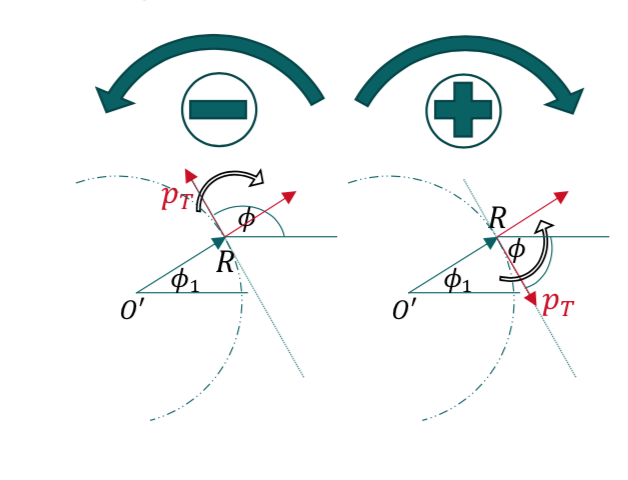
\includegraphics[width=0.7\linewidth]{Figures/rotations.png}
	\caption{Schematic representation of the determination of $\varphi_1$. Here the act of rotation is represented in blue.}
\end{figure}\\
In mathematical terms, let $\hat{\boldsymbol{p}}_T$ be the normalised 3-momentum vector projected to the XY-plane at $t=0$ for a positive particle. Then, the radial vector $\hat{\boldsymbol{r}}$ can be written with the rotation matrix $\textbf{R}_z (\phi)$ for an angle $\phi = \frac{\pi}{2}$ as
\begin{equation}
	\hat{\boldsymbol{r}} = \boldsymbol{R}_z\left(\phi = \frac{\pi}{2}\right)\,\hat{\boldsymbol{p}}_T = \begin{pmatrix}
	0 & -1 \\ 
	1 & 0 
	\end{pmatrix} \begin{pmatrix}
	\cos\varphi\\ 
	\sin\varphi
	\end{pmatrix} = \begin{pmatrix}
	-\sin\varphi\\ 
	\cos\varphi
	\end{pmatrix},
\end{equation}
so that the angle $|\varphi_1|$ between $\hat{\boldsymbol{r}}$ and the x-axis is given by the scalar product
\begin{center}
	\begin{tabular}{crl}
		&$\hat{\boldsymbol{r}} \cdot \boldsymbol{e}_x=$&$ -\sin\varphi= 1 \cdot 1\cdot\cos(|\varphi_1|)$\\
		\rule{0pt}{3ex}$\Rightarrow$&$\varphi_1 =$&$ \arccos(-\sin\varphi)\cdot(-\mathrm{sgn}(\hat{r}_y))$, \\ 
	\end{tabular} 
\end{center}
where the term $(-\mathrm{sgn}(\hat{r}_y))$ is due to the sign convention. Similarly, for a negatively charged particle, this yields
\begin{equation}
	\varphi_1 =\arccos(\sin\varphi)\cdot (-\mathrm{sgn}(\hat{r}_y)).
\end{equation}
The last two equations can be combined to obtain the relation between $\varphi_1$ and $\varphi$:
\begin{equation}
	\varphi_1 =\arccos(-\mathrm{sgn}(q)\sin\varphi)\cdot (-\mathrm{sgn}(\hat{r}_y))
\end{equation}
\paragraph{Finding \textbf{O'}}\mbox{}\\
In order to determine \textbf{O'}, one can use to the arbitrarily introduced parameter $t$ in the ansatz Eq. \ref{eq:ansatz}. Since the location of the particle is completely indifferent from the perspective of the IP-parameter problem, one can set the origin of time without any restrictions such that
\begin{equation}
	\boldsymbol{x}(0) = \boldsymbol{O'} +  \left(\begin{tabular}{c}
	$R\cos(\varphi_1) $\\ 
	$-R\sin(\varphi_1) $\\ 
	$0$\\
	\end{tabular} \right) \stackrel{!}{=} \boldsymbol{R}
\end{equation}
yielding
\begin{equation}
	\left\lbrace\begin{tabular}{ll}
	$O'_x =$&$R_x-R\cos(\varphi_1) $\\ 
	$O'_y =$&$R_y+R\sin(\varphi_1) $\\ 
	$O'_z =$&$R_z$\\
	\end{tabular} \right.
\end{equation}
which -- since $\varphi_1$ has already been found as a function of $\varphi$ and \textbf{R} is given by the fit algorithm -- is thereby uniquely defined.
\paragraph{Finding $v_z$}\mbox{}\\
Since the total momentum of the particle is given by $p = m\gamma v$, it follows
\begin{equation}
	v_z = \frac{p}{m\gamma}\cdot\cos\theta = \frac{p}{m\gamma}\cdot\cos\left(\frac{\pi}{2}-\lambda\right) =\frac{p}{m\gamma}\cdot -\sin(-\lambda) =  \frac{p}{m\gamma}\cdot\sin\lambda 
\end{equation}
\subsection{Results}
One way of judging the validity of a such theory is the comparison of the generator level dataset with the results obtained by this method on reconstruction level. This has been done in Fig. \ref{fig:deltaphinocut}, where the difference between the azimuthal angles $\Delta\phi$ between the IP on generator level and the differently reconstructed IP-vectors has been portrayed. In order to reduce uncertainties when dealing with such minimizer algorithms, this has been done with three different ones: the \verb|TMinimizer| of \verb|ROOT| utilises \verb|Minuit2|, a standard minimizer, the \verb|Brent|-algorithm, which is a combination of three different numerical minimizer algorithms (the bisection method, the secant method and the inverse quadratic interpolation). The third algorithm calculates an analytical solution by using a Taylor expansion of the helix for small $\omega t$-values, as discussed in Appendix \ref{AppendixA}, which delivers only approximative information about the overall distribution.
\begin{figure}[h]
	\centering
	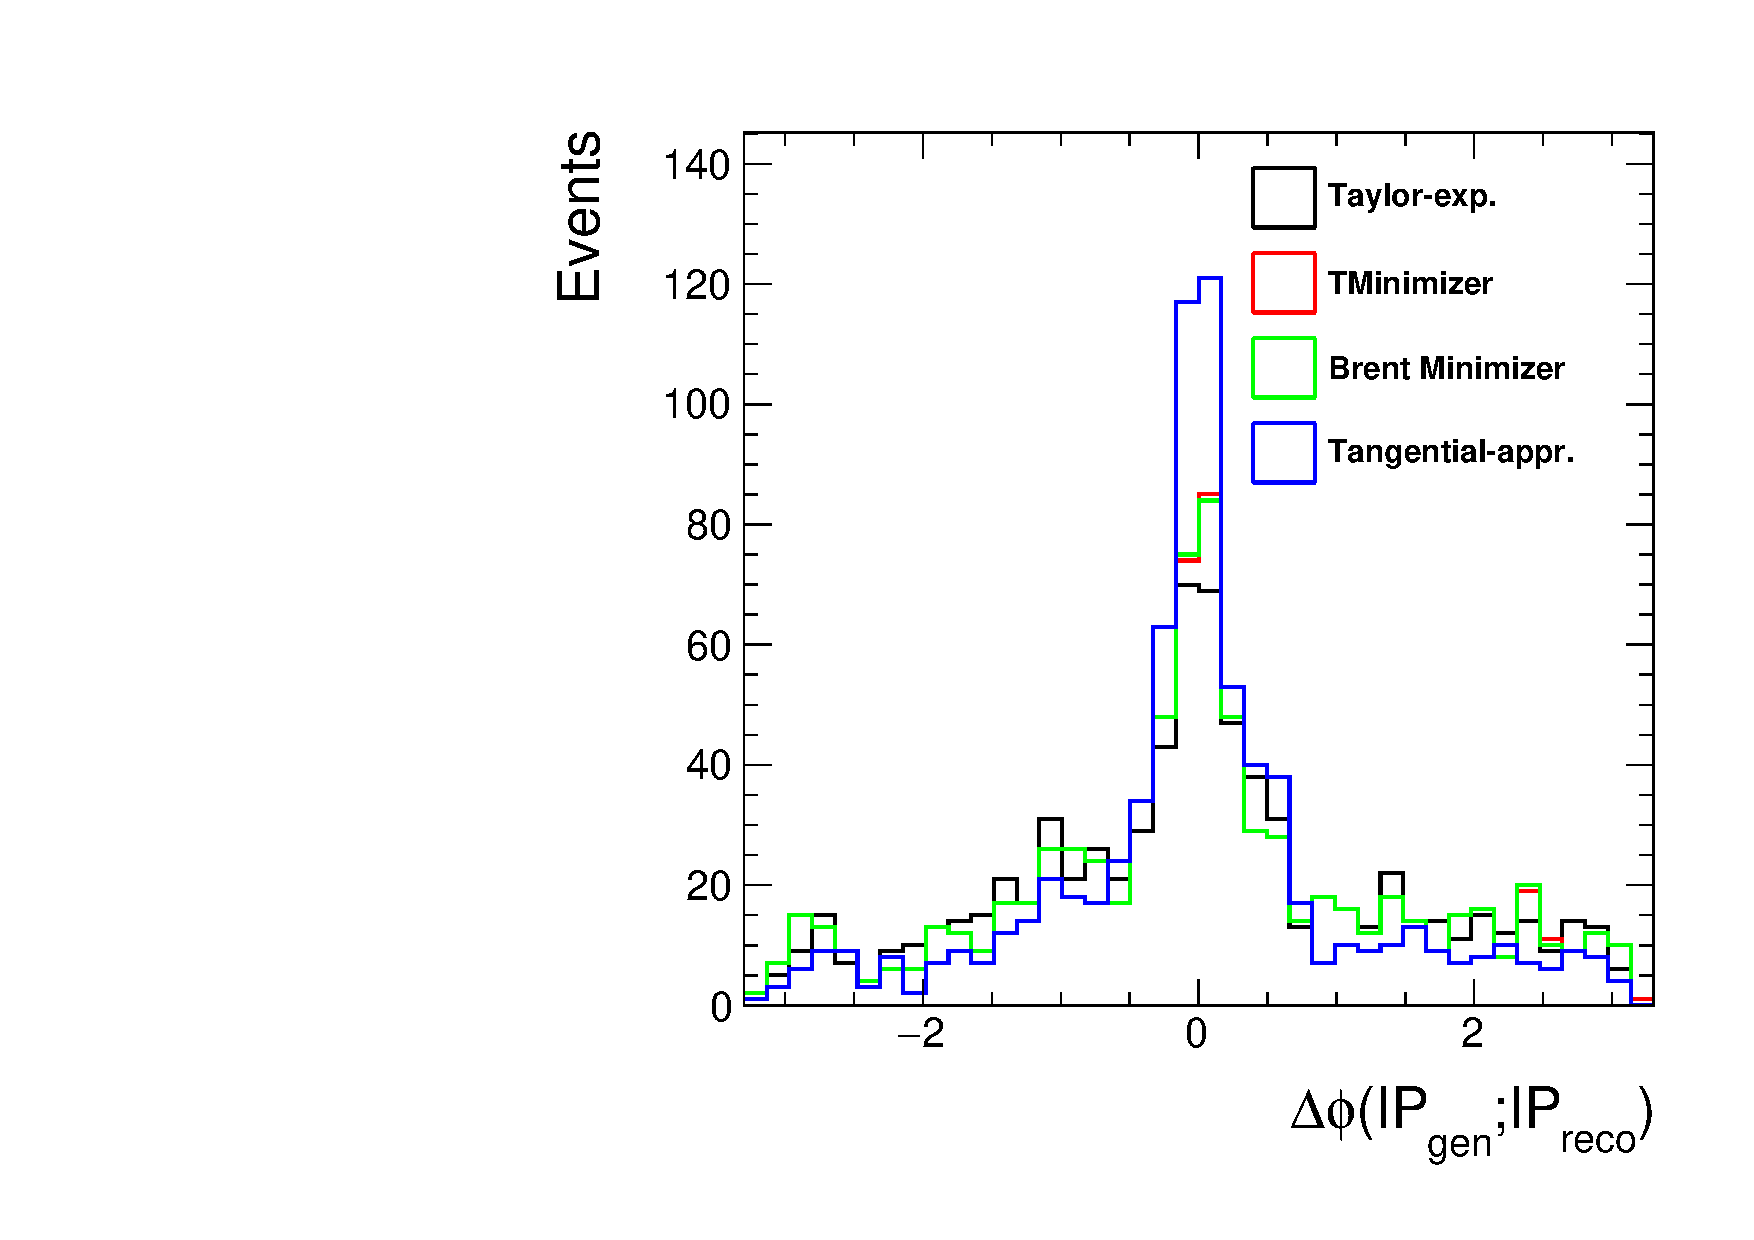
\includegraphics[width=0.7\linewidth]{Figures/deltaPhi_nocut}
	\caption{The comparison of generated and reconstructed IPs}
	\label{fig:deltaphinocut}
\end{figure}\\
For an algorithm performing better than the current tangential approximation, one expects a narrower distribution concerning $\Delta\phi$, since the data should deliver more reliable results. This is not the case however (no matter which numerical algorithm one considers meaning errors in the implementation can be excluded), which can be explained by the fact that the generated impact parameters are also calculated via the already discussed tangential approach.\\
While looking at these results, it is interesting to apply the cuts introduced in Chapter \ref{Chapter4}, which is portrayed in Fig. \ref{fig:deltaphicut}. Interestingly, a secondary peak arises around $\Delta\phi \approx -\pi/2$. This can be explained by the fact, that the primary vertex is not situated in the close neighbourhood of the origin, which can lead in some cases to systematic deviations in $\Delta\phi$.
\begin{figure}[h]
	\centering
	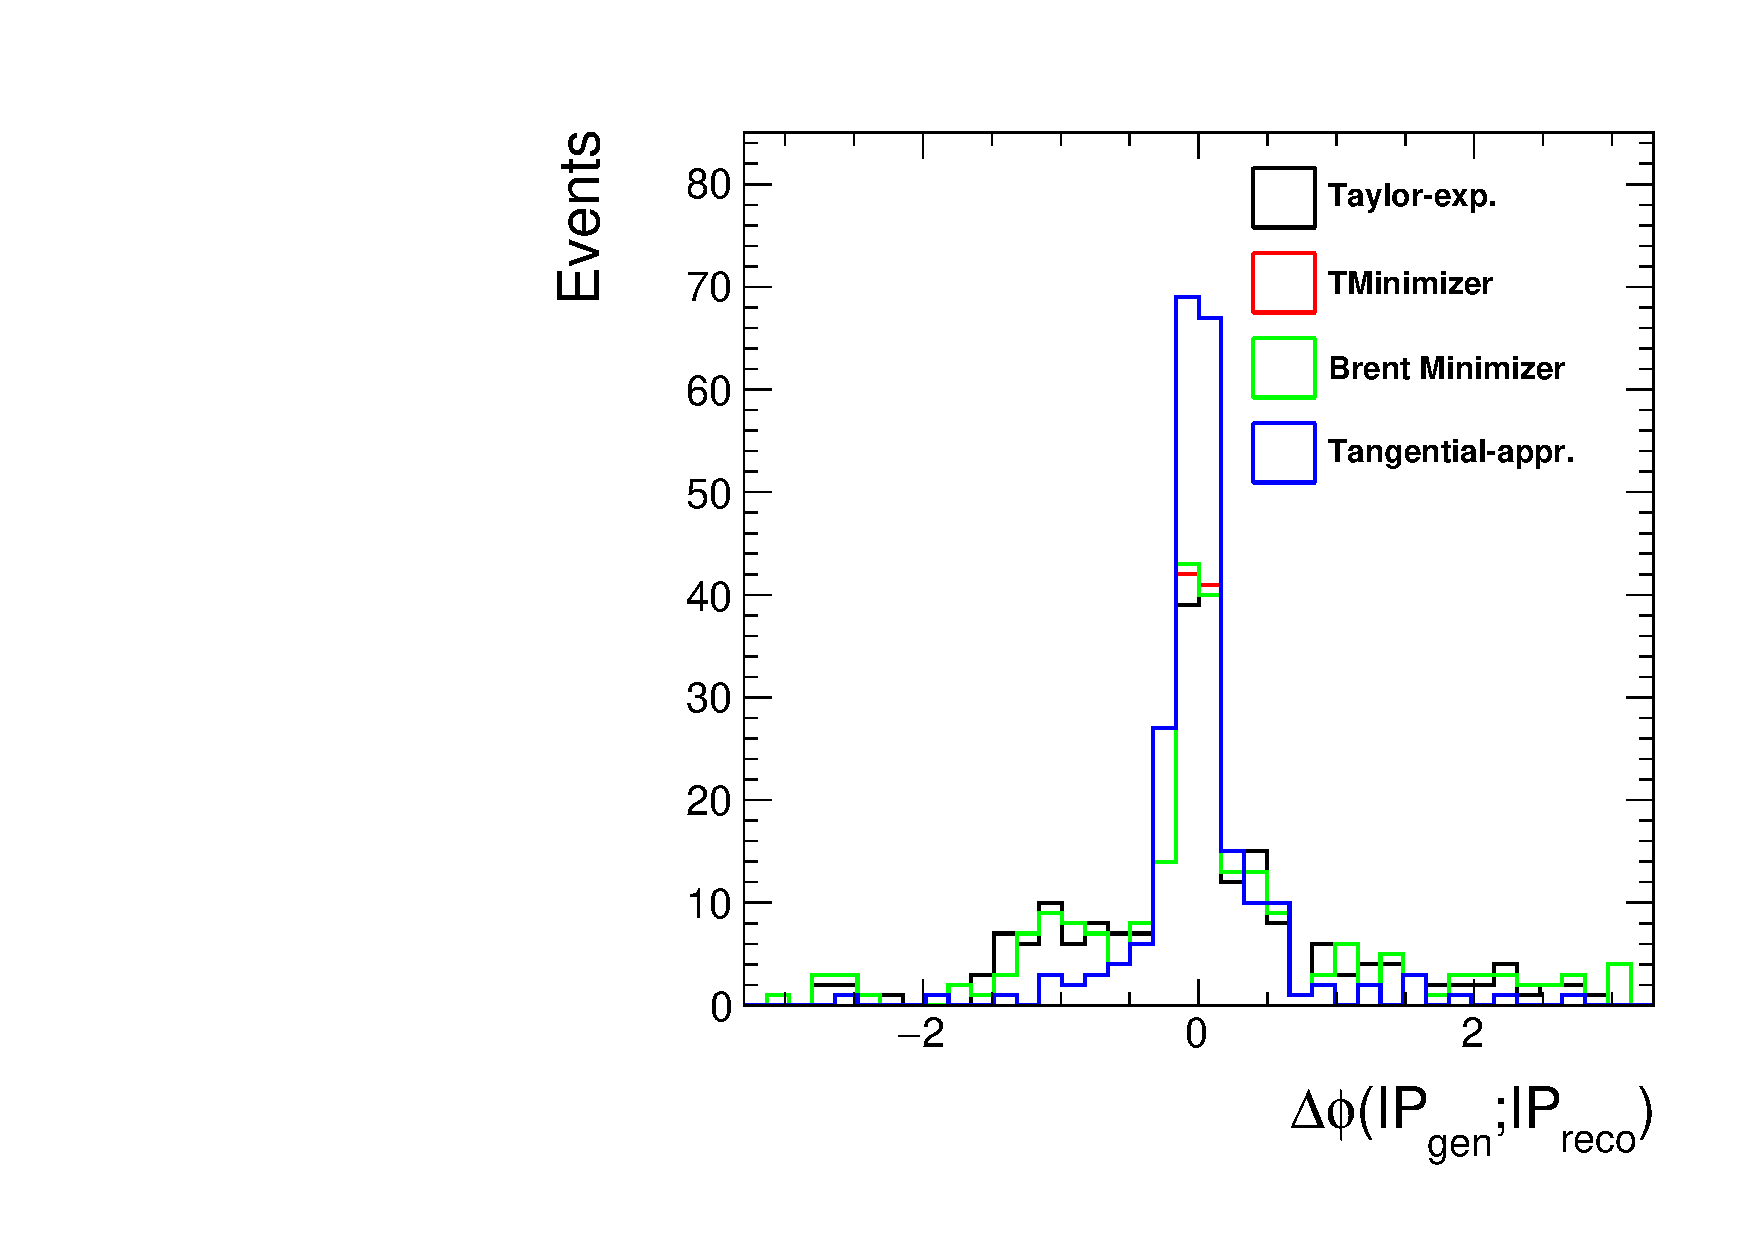
\includegraphics[width=0.7\linewidth]{Figures/deltaPhi_cut}
	\caption{The effect of cuts applied to the distribution of $\Delta\phi$. Here, only events with $d/\sigma_{\hat{d}} \geq 5$ were kept}
	\label{fig:deltaphicut}
\end{figure}

\subsection{Discussion of Validity}
In order to interpret and to see the validity of the helical approach, one has to take a look at the 2D geometry of the problem, shown in Fig. \ref{fig:geometry_diffIPs}, where $O$ corresponds to the origin of the coordinate system, \textbf{R} is the vector to the reference point (obtained from the track fit, being the closest point on the trajectory to $O$), $O'$ is the rotation centre of the helical trajectory and PV (SV) denote the primary (secondary) vertices respectively.
\begin{figure}[h]
	\centering
	\begin{tikzpicture}
	\centering
	
	\def\centerarc[#1](#2)(#3:#4:#5)% Syntax: [draw options] (center) (initial angle:final angle:radius)
	{ \draw[#1] ($(#2)+({#5*cos(#3)},{#5*sin(#3)})$) arc (#3:#4:#5); }
	
	\centerarc[<-](0,0)(60:90:8);
	\node[anchor = south] at ($({8*cos(60)},{8*sin(60)})$) {$l$};
	\centerarc[name path = h, dotted,line width=0.3mm, black](0,0)(90:160:8);
	\draw[densely dashed] (-5,8) --(5,8);
	\fill (0,0) circle (2pt) node[anchor=west] {O'};
	\draw[dashed] (0,0) --(0,8) node[anchor = east] at (0,4) {R};
	\fill (0,8) circle (1pt) node[anchor = south] {SV};
	\draw[line width=0.4mm,->] (0,8) -- (3,8) node[anchor=south east] {$p_T$};
	\draw[dashed,line width=0.4mm,->] (-3,5) -- (0,8) node[anchor = west] at (-1.5,6.5) {$\tau$};
	\draw[line width=0.6mm,->] (-3,5) -- (-3,8) node[anchor = west] at (-3,6.5) {$IP_{theo}$};
	\path [name path=OV] (-3,5) -- ++(-3,5);
	\draw [name intersections={of=OV and h, by=x}, ->] [very thick,blue] (-3,5) -- (x) node[below = 10pt] at (x) {$IP_{hel}$};
	\fill ($({6*cos(150)},{6*sin(150)})$) circle (2pt) node[anchor = north] {O};
	\draw[densely dashed, name path=tangent] ($({8*cos(150)},{8*sin(150)})$) --++($({8*sin(150)},{-8*cos(150)})$);
	\draw[dashed] ($({8*cos(150)},{8*sin(150)})$) -- ++ ($({-3*sin(150)},{3*cos(150)})$);
	\draw[line width=0.6mm,->] ($({6*cos(150)},{6*sin(150)})$)--($({8*cos(150)},{8*sin(150)})$)  node[anchor = east] {R};
	\path [name path = V_orth_to_tangent] (-3,5) --++($({6*cos(150)},{6*sin(150)})$);
	\draw [name intersections={of=V_orth_to_tangent and tangent, by=x}, ->] [very thick,red] (-3,5) -- (x) node[left = 1pt] at (x) {$IP_{tan}$};
	\fill (-3,5) circle (2pt) node[anchor=north] {PV};
	\end{tikzpicture}
	\caption{Visualisation of the IPs obtained by different algorithms in the 2D case.}
	\label{fig:geometry_diffIPs}
\end{figure}\\
In this graph, one can immediately see that in cases where the primary vertex is far from the origin $O$, the tangential approach becomes meaningless. In addition, one can see the extreme effect of displacement of the IP-vector due to the introduction of the reference point $R$, the angle between the theoretical and the reconstructed IP having approximately doubled. Let alone this would be enough reason to omit the previous approach and to look for an alternative.\\
On the other hand, the fact of ignoring the arbitrarily introduced point \textbf{R} should deliver better results, which would have manifested in a narrower distribution. Nevertheless, each IP-vector on generator level have also been calculated with the tangential approach, meaning the "true" impact parameters on generator level are missing. For this reason, a further comparison of this method with the "exact" IPs is necessary.\\
The root of the problem lies within the fact, that the $\tau$-particles coming from primary vertex cannot be fully reconstructed, or equivalently, the secondary vertex can only be reconstructed at the cost of great uncertainties. For this reason, one could also execute a kinematical fit with respect to the $\tau$ leptons in order to determine the location of the SV, from which, by minimizing the distance between the PV and the tangent defined by the 3-momentum of $l$, the correct IP-vector can be obtained. However, this goes beyond the scope of this thesis.